
\section{Обзор предметной области}

\subsection{Обзор аналогов разрабатываемого продукта}
\subsection{Математическая модель квадрокоптера}

Для понимания принципов полета квадрокоптера рассмотрим его математическую модель в двух системах координат (СК):

1. Неподвижная система координат (НСК), в качестве которой выступает нормальная земная система координат с заданными перпендикулярными друг другу координатными осями \(O_{g}X_{g}\), \(O_{g}Y_{g}\), и \(O_{g}Z_{g}\), причем ось \(O_{g}Z_{g}\) направлена противоположно вектору силы тяжести.

2. Связанная с квадрокоптером система координат (ССК), центр которой размещен в центре масс аппарата, а оси \(OX\), \(OY\), и \(OZ\) параллельны и сонаправлены с осями неподвижной системы. Угловое положение аппарата зададим тремя углами Эйлера: углами крена \(\phi\), тангажа \(\theta\) и рыскания \(\psi\), определяющими вращение вокруг осей \(OX\), \(OY\), и \(OZ\) соответственно. Основываясь на ранее рассмотренных системах координат можно утверждать о том, что квадрокоптер имеет шесть степеней свободы, а именно три линейных координаты \([x; y; z ]\) и три угловых \([\theta, \phi, \psi]\). В качестве управляющих каналов выступают скорости вращения роторов (рисунок \ref{fig:ris1}), которые создают динамику движения БПЛА в пространстве. Возникающие в результате подачи управляющих воздействий силы и моменты пропорциональны квадрату угловых скоростей винтов \(\Omega^2\). Поэтому, для достижения желаемого режима работы БПЛА, необходимо связать совокупность управляющих воздействий со степенями свободы БПЛА, через уравнения связи, которые определяют основные режимы движения квадрокоптера в пространстве.
% ~\ref{fig:ris1}
\begin{figure}[H]
	\centering
	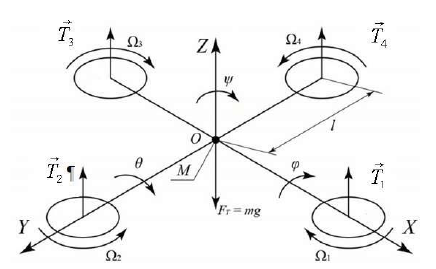
\includegraphics[width=0.5\linewidth]{../RW/pics/ris1}
	\caption{Связанная система координат квадрокоптера
	}
	\label{fig:ris1}
\end{figure}

В качестве первого режима БПЛА \(U_{1}\) рассмотрим движение вдоль оси \(OZ\), принадлежащей ССК. Данное движение обеспечивается одновременным увеличением скоростей винтов на одинаковое значение угловой скорости \(\Delta a\). Полученное при этом движение характеризуется взлетом или посадкой квадрокоптера (при нулевых значениях тангажа и крена) и описывается следующим выражением:
\begin{equation}
U_{1}=b(\Omega_{1}^2+\Omega_{2}^2+\Omega_{3}^2+\Omega_{4}^2)
\end{equation}

где \(b\) -- аэродинамическая составляющая тяги винта.
В качестве второго режима движения БПЛА \(U_{2}\) необходимо взять поворот вокруг оси \(OX\), принадлежащей ССК. Данное движение достигается путем увеличения/уменьшения на величину \(\Delta a\) значения \(\Omega_{4}\) левого винта и уменьшением/увеличением на величину \(\Delta b\) значения \(\Omega_{1}\)
правого. Полученное при этом движение характеризуется изменением угла крена \(\phi\) и описывается следующим выражением:
\begin{equation}
U_{2}=lb(-\Omega_{2}^2-\Omega_{4}^2)
\end{equation}

где \(l\) -- расстояние между центром квадрокоптера и центром винта.

В качестве третьего режима движения \(U_{3}\) необходимо взять поворот БПЛА вокруг оси \(OY\), принадлежащей ССК. Данное движение достигается путем уменьшения / увеличения на величину \(\Delta a\) значения \(\Omega_{1}\) фронтального винта и увеличения / уменьшения на величину \(\Delta b\) значения \(\Omega_{3}\) заднего. Полученное при этом движение характеризуется изменением угла тангажа \(\theta\) и описывается следующим выражением:
\begin{equation}
U_{3}=lb(-\Omega_{1}^2-\Omega_{3}^2)
\end{equation}

В качестве последнего, четвертого, режима движения \(U_{4}\) необходимо взять поворот БПЛА вокруг оси \(OZ\), принадлежащей ССК. Данное движение достигается путем одновременного увеличения/уменьшения на величину \(\Delta a\) значений \(\Omega_{4}\) левого и \(\Omega_{2}\) правого винтов, а также одновременного уменьшения / увеличения на величину \(\Delta b\) значений \(\Omega_{1}\) фронтального и \(\Omega_{3}\) заднего винтов. Благодаря вращению роторов в диагонально противоположных направлениях, полученное движение характеризуется изменением угла рыскания \(\psi\) и описывается следующим выражением:
\begin{equation}
U_{4}=d(-\Omega_{1}^2+\Omega_{2}^2-\Omega_{3}^2+\Omega_{4}^2)
\end{equation}
где \(d\) -- аэродинамическая составляющая коэффициента сопротивления среды.
Введенное с учетом (1) -- (4) множество \(U\), характеризующее режимы
движения квадрокоптера, можно записать следующим образом:

\begin{equation}
U = \left\{ \begin{aligned}
U_{1}&=&b(\Omega_{1}^2+\Omega_{2}^2+\Omega_{3}^2+\Omega_{4}^2)\\
U_{2}&=&lb(-\Omega_{2}^2-\Omega_{4}^2)\\
U_{3}&=&lb(-\Omega_{1}^2-\Omega_{3}^2)\\
U_{4}&=&d(-\Omega_{1}^2+\Omega_{2}^2-\Omega_{3}^2+\Omega_{4}^2)
\end{aligned} \right.
\end{equation}

Множество \(U\) определяет связь между системой исполнительных приводов и платформой БПЛА \cite{mathmodel}.

\subsection{Устройство квадрокоптера}
Далее рассмотрим компонентную базу квадрокоптера.

Квадрокоптер -- беспилотный летательный аппарат мультироторного типа с четырьмя несущими ВМГ (условная схема представлена на рисунке \ref{fig:pix}).
Квадрокоптер состоит из:
\begin{itemize}
	\item рамы;
	\item 4 моторов, пропеллеров (винто -- моторная группа, далее ВМГ);
	\item 4 регуляторов оборотов (далее рассматривается как часть ВМГ);
	\item полетного контроллера;
	\item аккумулятора;
	\item камеры, видеопередатчика, видеоантенны (опционально для FPV);
	\item радиоприемника (радиопередатчика, если необходима отправка телеметрии);
	\item другой периферии (например, GPS, магнитометр, дальномер, телеметрийный модуль).
	\item EmuFlight.
\end{itemize}

 % ~\ref{fig:pix}
 \begin{figure}[H]
 	\centering
 	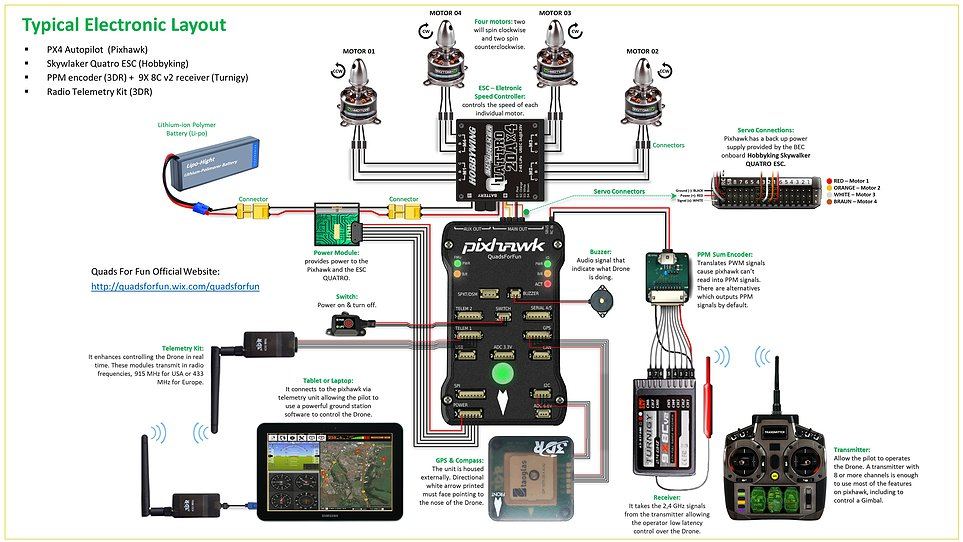
\includegraphics[width=0.5\linewidth]{../RW/pics/pix}
 	\caption{Пример схемы подключения
 	}
 	\label{fig:pix}
 \end{figure}

Рассмотрим каждый компонент с его характеристиками подробнее.

%винты должжны вмещаться и не создавать турбулентный поток
Рама - несущий компонент, на котором располагается вся электроника квадрокоптера. Рама должна быть жесткой, прочной, и в то же время легкой. На данный момент лучшим материалом для рам квадрокоптеров является карбон.

Компоненты ВМГ подбираются в зависимости от поставленных задач и характеристик БПЛА. Для современных БПЛА используются моторы бесколлекторного типа. Основными их характеристиками являются размер и количество оборотов на вольт.
Диаметр, шаг и количество лопастей пропеллера определяют тягу квадрокоптера. При этом пропеллеры с большим шагом обеспечивают большую скорость полета.

Регулятор принимает управляющий сигнал с полетного контроллера и на его основе задает обороты моторов. В случае мотора бесколлекторного типа это происходит путем открытия силовых ключей (мосфетов) для коммутации обмоток.

Полетный контроллер -- система реального времени, которая интерпретирует входящие данные от приемника и бортовых датчиков (гироскопа, акселерометра, барометра и др.), на основе которых рассчитывает положение квадрокоптера и производит регулирование путем выдачи управляющего сигнала на ВМГ. Все алгоритмы работы полетного контроллера содержатся в прошивке -- программном обеспечении, которое выбирается в зависимости от схемы полетного контроллера и поставленных задач.

Для питания квадрокоптера используются литий-полимерные и литий-ионные аккумуляторы. В зависимости от задач и размеров подбирается количество ячеек аккумулятора, емкость и токоотдача.

Видеосистема состоит из трех основных компонентов: камера, видеопередатчик, приемник, передающая и принимающая антенны. Видеопередатчик, в большинстве случаев, функционирует на диапазоне частот 5.8 ГГц.

Для осуществления контроля над квадрокоптером используется радиоуправление. Для приема сигнала к полетному контроллеру подключается приемник, общающийся с передатчиком по определенному протоколу на указанном диапазоне частот. Информация с датчиков квадрокоптера оператору может передаваться с помощью устройств приема-передачи телеметрии.

Также на квадрокоптер ставится бортовой компьютер для выполнения более высокоуровневых вычислительных задач, например, когда необходима обработка видеопотока или выполнение других высокоуровневых вычислительных задач. Как правило, бортовой компьютер представляет собой микрокомпьютер, например, Ras\-pber\-ry Pi или Nvi\-dia Jet\-son. 

Теперь разберем, какие есть прошивки для полетных контроллеров.

\subsection{Семейства прошивок полетного контроллера}
Ввиду того, что нам может потребоваться доработка функционала прошивки полетного контроллера, мы не будем рассматривать прошивки с закрытым исходным кодом. Наряду с функционалом прошивки одним из ключевых факторов ее выбора будет тип открытой лицензии. Если взять во внимание наиболее популярные открытые прошивки для полетных контроллеров, то можно выделить 2 семейства: потомки MultiWii и прошивки под полетные контроллеры семейства PixHawk.

MultiWii - прошивка, изначально разработанная для получения и обработки данных с гироскопов и акселерометров игровой консоли Nintendo Wii. Позже, на основе частей из консоли Nintendo Wii (акселерометр + гироскоп) и контроллера atmega, был спроектирован полетный контроллер, на который была установлена уже коптерная прошивка MultiWii \cite{multiwii}. Со временем платформа atmega перестала удовлетворять аппаратным критериям, и MultiWii перерос в BaseFlight, базирующийся на чипах семейства STM32, а он в свою очередь в CleanFlight. Разработчики CleanFlight разошлись во мнениях касаемо функционала прошивки и сделали следующие ответвления:
\begin{itemize}
	\item BetaFlight;
	\item INav;
	\item EmuFlight.
\end{itemize}

BetaFlight нацелен на гоночные квадрокоптеры. Основными особенностями являются: минимальная фазовая задержка, точное следование управляющему сигналу (setpoint) и поддержка огромного количества полетных контроллеров (target).
Стоит пояснить фразу "минимальная фазовая задержка". При фильтрации показаний гироскопа происходит сдвиг по фазе между исходным и фильтрованным сигналами, что приводит к запозданию реакции ПИД регулятора, и как итог -- ПИД осцилляции. Фильтры в BetaFlight оптимизированы для уменьшения фазовой задержки.

INav сфокусирован на навигационных возможностях. Позволяет выполнять полеты по точкам, исходя из данных, полученных периферией. Поддерживает различные платформы, включая БПЛА мультироторного и самолетного типов, сухопутные и водные управляемые модели.

EmuFlight предназначен для акробатических и кинематографических полетов. Позволяет настроить квадрокоптер на плавный полет, содержит множество алгоритмов для фильтрации шумов.

Среди описанных прошивок только INav имеет функционал для автономных полетов, но инструменты внешнего управления имеют весьма скудный функционал, потому такой вариант не подходит для решения поставленной задачи.

В семействе полетных контроллеров PixHawk наиболее популярны прошивки PX4 и Ardupilot. Эти прошивки активно используются как хоббистами, так и для решения профессиональных задач в промышленности и сфере эксплуатации БАС. Практически весь их функционал нацелен на выполнение автономных миссий. Ardupilot, в основном, разрабатывается и используется хоббийным сообществом. PX4 изначально был студенческой учебно-исследовательской работой, но сейчас его используют исследователи в области программирования, стабилизации и навигации БПЛА во всем мире.

Изначально это был студенческий НИР, но спустя 3 года вышел официальный релиз, сейчас его используют исследователи в области программирования, стабилизации и навигации БПЛА во всем мире. Главными особенностями PX4 являются поддержка огромного количества датчиков и навигация в режиме OFFBOARD, который позволяет управлять беспилотником при помощи бортового компьютера. OFFBOARD режим PX4 предоставляет огромные возможности для конфигурирования и управления полетным заданием с внешнего устройства, что подходит для поставленной задачи. Рассмотрим PX4 подробнее.

\subsubsection{PX4}
%\url{https://docs.px4.io/master/en/getting_started/px4_basic_concepts.html}
%\url{https://docs.px4.io/master/en/contribute/licenses.html}
%https://docs.px4.io/master/en/simulation/#simulator-mavlink-api

PX4 - прошивка с открытым исходным кодом, публикуемая под лицензией BSD-3-Clause. PX4 позволяет управлять различными типами беспилотников, включая: летательные (мультикоптеры, самолеты и вертолеты), наземные и подводные аппараты. Он совместим с большим количеством оборудования, датчиков и другой периферии. Позволяет реализовать гибкие режимы полета и функции безопасности.
Параметры PX4 настраиваются с помощью Q\-Ground\-Control \cite{px4}.

QGroundControl - кросплатформенный конфигуратор для настройки PX4 и Ardupilot прошивок. Он обеспечивает полное управление полетом и настройку беспилотника \cite{qgroundcontrol}.

PX4 для определения состояния аппарата, его стабилизации и автономного полета использует датчики, такие как: гироскоп, акселерометр, магнитометр (компас) и барометр. Для включения всех автоматических режимов и некоторых вспомогательных требуется GPS или другая система позиционирования.
Для передачи данных / телеметрии между наземной станцией управления, такой как Q\-Ground\-Control, и беспилотником, работающим под управлением PX4 может использоваться как проводное, так и беспроводное соединение по протоколу MAVLink. Он позволяет настраивать параметры во время полета, проверять телеметрию в режиме реального времени, менять миссию на лету и т. д.

PX4 можно управлять с отдельного компьютера через кабель или Wi-Fi. Дрон и компьютер обычно обмениваются данными с помощью API MAVLink, такого как MAVSDK или MAVROS \cite{px4}.

\subsection{MAVLink}

%\url{https://mavlink.io/en/}

MAVLink -- это протокол двоичной телеметрии, разработанный для систем с ограниченными ресурсами и каналов с ограниченной пропускной способностью. MAVLink был впервые выпущен в начале 2009 года Лоренцем Мейером (основателем PX4) и в настоящее время имеет значительное количество разработчиков. Протокол развернут в двух основных версиях: v1.0 и v2.0, которые имеют обратную совместимость (реализации v2.0 могут анализировать и отправлять пакеты v1.0).

MAVLink реализует гибрид шаблонов проектирования взаимодействия «публикация -- подписка» и «точка -- точка». В этом гибридном шаблоне потоки данных отправляются / публикуются как темы, а подпротоколы конфигурации, такие как протокол задания или протокол параметров, реализуются шаблоном «точка-точка» с повторной передачей.

Сообщения определяются в файлах XML. Каждый файл XML определяет набор сообщений, поддерживаемый MAVLink системой, также называемый «диалектом». Набор эталонных сообщений, который реализуется большинством наземных станций управления и автопилотов, определен в common.xml (большинство диалектов основано на этом определении).

Набор инструментов MAVLink использует определения XML сообщений для генерации библиотеки MAVLink для каждого из поддерживаемых языков программирования. Дроны, наземные станции управления и другие системы MAVLink используют сгенерированные библиотеки для связи. Они распространяются под лицензией MIT и поэтому могут использоваться без ограничений в любом приложении с закрытым исходным кодом без публикации исходного кода. MAVLink был впервые выпущен в начале 2009 года Лоренцем Мейером (основателем PX4) и в настоящее время имеет значительное количество разработчиков \cite{px}.

MAVLink поддерживает множество языков программирования, работающих на множестве микроконтроллеров / операционных систем (включая ARM7, ATMega, dsPic, STM32 и Windows, Linux, MacOS, Android и iOS). Допускает одновременно до 255 систем в сети (беспилотники, наземные станции и т. д.)

Обеспечивает как внешнюю, так и бортовую связь (например, между q\-ground\-con\-trol и дроном, а также между автопилотом дрона и камерой дрона с поддержкой MAVLink) \cite{mavlink}.

MAVLink развернут в двух основных версиях: v1.0 и v2.0, которые имеют обратную совместимость (реализации v2.0 могут анализировать и отправлять пакеты v1.0). Потоки телеметрических данных отправляются в многоадресном режиме, в то время как аспекты протокола, которые изменяют конфигурацию системы и требуют гарантированной доставки, являются point-to-point с повторной передачей.

%//переделать

Для того, чтобы запускать на наземной станции автономные миссии для БПЛА, необходим набор инструментов, позволяющий обрабатывать MAVLink сообщения, преобразовывать показания с камеры в координаты положения квадрокоптера и отправлять управляющие команды квадрокоптеру. Для выполнения обозначенного функционала можно использовать робототехнические фреймворки. Наиболее популярным робототехническим фреймворком является ROS.
% дописать про офборд
\subsubsection{Структура пакета}
Ключевая особенность разрабатываемого ПАК в том, что вся необходимая для управления информация будет передаваться с помощью протокола MAVLink через средства приема-передачи телеметрии по воздуху, в то время как существующие решения передают информацию через UART.

Рассмотрим подробнее устройство MAVLink. Ниже приведена структура пакета MAVLink v2. Представление в памяти может отличаться.

uint8\_t magic;              //Метка начала

uint8\_t len;                //Размер данных / длина полезной нагрузки (сообщения)

uint8\_t incompat\_flags;     //Обратно несовместимые флаги

uint8\_t compat\_flags;       //Обратно совместимые флаги

uint8\_t seq;                //Порядковый номер сообщения для выявления потери сообщения

uint8\_t sysid;              //ID системы-отправителя

uint8\_t compid;             //ID компонента-отправителя

uint8\_t msgid 0:7;          //ID сообщения (первый байт), от него зависит, какие данные будут лежать в полезной нагрузке пакета

uint8\_t msgid 8:15;         //ID сообщения (второй байт)

uint8\_t msgid 16:23;        //ID сообщения (третий байт)

uint8\_t payload[max 255];   //Полезная нагрузка (размер сообщения максимум 255 байт) 

uint16\_t checksum;          //Контрольная сумма

uint8\_t signature[13];      //Сигнатура (опционально)

Структура пакета MAVLink v1 аналогична, но опускает incompat\_flags, compat\_flags и signature, и имеет только один байт для адреса сообщения \cite{mavlink}.

%https://mavlink.io/en/about/overview.html
\subsubsection{Публикация}
Беспроводной формат MAVLink оптимизирован для систем с ограниченными ресурсами и, следовательно, порядок полей не такой, как в спецификации XML. Все поля сообщения сортируются по размеру, сначала с самыми большими полями (uint64\_t), а затем с меньшими полями. Сортировка выполняется с использованием стабильного алгоритма сортировки, который гарантирует, что любые поля, которые не нужно переупорядочивать, останутся в том же порядке. Это предотвращает проблемы с выравниванием в системах кодирования / декодирования и позволяет очень эффективно упаковывать / распаковывать данные \cite{mavlink}.

Примеры MAV\-Link-сообщений:

ATTITUDE, ATTITUDE\_QUATERNION – ориентация квадрокоптера в пространстве;

LOCAL\_POSITION\_NED – локальная позиция квадрокоптера;

GLOBAL\_POSITION\_INT – глобальная позиция квадрокоптера (широта / долгота / высота);

COMMAND\_LONG – команда для квадрокоптера (взлететь, сесть, переключить режим и т. д.) \cite{clover}.

\subsubsection{Многоадресные потоки и гарантированная доставка}
MAVLink создан для систем, в которых высокоскоростные потоки данных от беспилотников поступают в наземные станции, но смешиваются с передачами, требующими гарантированной доставки. Ключевой момент состоит в том, что для большинства потоков телеметрии не существует известного или единственного получателя: вместо этого, как правило, наземная станция управления нуждаются в одном и том же потоке данных.
С другой стороны, настройка бортовой миссии или изменение конфигурации системы с бортовыми параметрами требует точка -- точка связи с гарантированной доставкой. MAVLink достигает очень высокой эффективности за счет использования обоих режимов работы.

\subsubsection{Соединение точка -- точка}
В режиме точка -- точка при изменении миссии, параметры и передаче команд MAV\-Link использует идентификатор цели и целевой компонент \cite{mavlink}.

\subsubsection{Режим топиков (публикация-подписка)}
В режиме топиков протокол не будет выдавать идентификатор целевой системы и компонента для сообщений, чтобы сэкономить пропускную способность канала. Типичными примерами этого режима связи являются все потоки данных автопилота, такие как положение, координаты и т. д.

Основное преимущество этого режима заключается в том, что не создаются дополнительные накладные расходы, и все подписчики могут получать эти данные.

Для наших целей MAVLINK полезен тем, что позволяет получать практически всю информации о внутреннем состоянии полетного контроллера и передавать ему на вход управляющие сигналы. Управляющие сигналы могут быть как в виде указания положения стиков радиоаппаратуры, так и в виде задания угловых скоростей для квадрокоптера. Самым верхнеуровневым типом команды является указание требуемой позиции с предоставлением полетному контроллеру самостоятельного выбора способа достижения этой позиции. Таким образом, мы можем очень точно управлять положением квадрокоптера.

\subsection{ECL EKF}
Библиотека оценки и управления (ECL) использует алгоритм расширенного фильтра Калмана (EKF) для обработки измерений датчика и предоставления оценки следующих состояний:
\begin{itemize}
	\item кватернион, определяющий вращение из одной системы отсчета (North, East, Down локальной координатной плоскости) в другую ( X, Y, Z тела);
	\item скорость на IMU - North, East, Down (м / с);
	\item положение в IMU - North, East, Down (м);
	\item оценки смещения угла дельты IMU - X, Y, Z (рад);
	\item оценки смещения дельта-скорости IMU - X, Y, Z (м / с);
	\item компоненты магнитного поля Земли - North, East, Down (гаусс);
	\item смещение магнитного поля рамы кузова автомобиля - X, Y, Z (Гаусс);
	\item скорость ветра - север, восток (м / с).
\end{itemize}

EKF реализует систему <<отложенного временного горизонта слияния>>, что позволяет учесть временные задержки опроса датчиков относительно IMU. Данные для каждого датчика буферизуются FIFO и извлекаются из буфера с помощью EKF для использования в нужное время. Компенсация задержки для каждого датчика регулируется параметрами EKF2*DELAY.

EKF имеет разные режимы работы, которые позволяют использовать различные комбинации опроса датчиков. При запуске фильтр проверяет минимальную жизнеспособную комбинацию датчиков и после завершения начального выравнивания наклона, рыскания и высоты входит в режим, который обеспечивает оценку вращения, вертикальной скорости, вертикального положения, отклонения угла отклонения IMU и отклонения дельта-скорости IMU.

Для этого режима требуются данные IMU, источник рыскания (магнитометр или система внешнего визуального позиционирования (external vision)) и источник данных о высоте. Этот минимальный набор данных требуется для всех режимов работы EKF. Затем данные других датчиков можно использовать для оценки дополнительных состояний \cite{px4}.

\subsection{Robotic Operating System}
%\url{https://www.ros.org/about-ros/}

Robotic Operating System (далее ROS) -- это гибкая платформа для написания программного обеспечения для роботов; набор инструментов, библиотек и соглашений, которые призваны упростить задачу создания сложного и надежного поведения роботов на самых разных роботизированных платформах \cite{ros}.

Целью создания ROS является создание среды разработки, которая позволяет разработчикам ПО для роботов взаимодействовать на глобальном уровне.

ROS сосредоточена на максимизации повторного использования кода при разработке. Основные характеристики, позволяющие это реализовать:

Распределенные процессы. Структура ROS создана в виде минимальных единиц исполняемых процессов (нод), и каждый процесс выполняется изолированно. Взаимодействие разных нод происходит только на уровне обмена сообщениями.

Управление пакетами. Несколько процессов, имеющих общую задачу, объединяются в пакеты. Управление пакетами подразумевает набор утилит, позволяющих автоматически скачивать, устанавливать и удалять пакеты. Пакетный менеджер гарантирует работоспособность и целостность установленных пакетов.

Публичные репозитории и документация. Каждый доступный пакет публикуется в публичном репозитории. Документация пакетов публикуется в единой системе, которая упрощает поиск необходимых пакетов.

Единое API. При разработке программы, использующей ROS, вы получаете простое и легко встраиваемое API. При этом при использовании API нет разницы, на каком языке была написана программа.

Поддержка различных языков программирования. ROS предоставляет клиентские библиотеки для поддержки различных языков программирования. Наиболее популярны Python, C ++, а также такие языки, как Lisp, JAVA, C\#, Lua и Ruby \cite{voltbro}.

Рассмотрим концепции ROS: ноды, топики, сервисы.

\subsubsection{Ноды}
Нода представляет собой процесс, который выполняет вычисления. Ноды объединяются в граф и взаимодействуют друг с другом с помощью топиков, сервисов и сервера параметров. Ноды предназначены для работы в мелкомасштабном масштабе; система управления роботом обычно состоит из множества нод.

Все ноды имеют имя ресурса графа, которое однозначно идентифицирует их для остальной системы. Ноды также имеют типы, который упрощает процесс обращения к исполняемому файлу узла в файловой системе. Эти типы представляют собой имена ресурсов пакета с именем пакета ноды и именем исполняемого файла ноды. Чтобы определить тип ноды, ROS ищет все исполняемые файлы в пакете с указанным именем и выбирает первый из найденных \cite{ros}. 
% http://wiki.ros.org/Nodes \cite{ros}

%ROS-нода – это специальная программа (обычно написанная на Python или C++), которая взаимодействует с другими нодами посредством ROS-топиков и ROS-сервисов. Разделение сложных робототехнических систем на изолированные ноды дает определенные преимущества: понижается связанность кода, повышается переиспользуемость и надежность.

Очень многие робототехнические библиотеки и драйвера выполнены в виде ROS-нод.
Для того, чтобы преобразовать обычную программу в ROS-ноду, необходимо подключить к ней библиотеку rospy или roscpp и добавить инициализирующий код.

Пример ROS-ноды на языке Python представлен в листинге \ref{lst:1}:

\begin{Program}[H]
	\caption{Пример ROS-ноды на языке Python} \label{lst:1}
\begin{MyCode}
	import rospy
	
	rospy.init_node('my_ros_node')  # имя ROS-ноды
	
	rospy.spin()  # входим в бесконечный цикл...
\end{MyCode}
\end{Program}

Возможность запуска нескольких нод в одном процессе осуществляет пакет nodelet. Он позволяет производить обмен сообщений внутри процесса без затрат на копирование \cite{ros}.
%http://wiki.ros.org/nodelet

\subsubsection{Топики}
Топиками называют шины, по которым ноды обмениваются сообщениями. Топики имеют семантику анонимной публикации/подписки, которая отделяет производство информации от ее потребления. Как правило, ноды не знают, с кем они общаются. Вместо этого ноды, которые заинтересованы в данных, подписываются на соответствующие топики; ноды, которые генерируют данные, публикуются в соответствующем топике. У топиков может быть несколько издателей и подписчиков.

Топики предназначены для однонаправленного потокового общения.

Каждый топик строго типизирован в соответствии с типом сообщения ROS, используемым для публикации в ней, и ноды могут получать сообщения только с совпадающим типом. Master не обеспечивает согласованность типа среди издателей, но абоненты не будут устанавливать сообщение транспорта, если топики не совпадают. Кроме того, все клиенты ROS проверяют совпадение MD5, вычисленного из файлов msg. Эта проверка гарантирует, что ноды ROS были скомпилированы из согласованных кодовых баз \cite{ros}. Пример публикации сообщения в топик на языке Python приведен в листинге \ref{lst:2}:
% http://wiki.ros.org/Topics

\begin{Program}[H]
	\caption{Пример публикации сообщения типа std\_msgs / String (строка) в топик foo на языке Python} \label{lst:2}
\begin{MyCode}
	from std_msgs.msg import String
	
	# создаем Publisher'а
	foo_pub = rospy.Publisher('/foo', String, queue_size=1)
	
	# публикуем сообщение
	foo_pub.publish(data='Hello, world!')
\end{MyCode}
\end{Program}

\begin{Program}[H]
	\caption{Пример подписки на топик /foo на языке Python} \label{lst:3}
\begin{MyCode}
	def foo_callback(msg):
	print msg.data
	
	#При получении сообщения в топик /foo
	#будет вызвана функция foo_callback.
	rospy.Subscriber('/foo', String, foo_callback)
\end{MyCode}
\end{Program}

Также существует возможность работы с топиками с помощью утилиты rostopic. Например, с помощью следующей команды можно просматривать сообщения, публикуемые в топик /mavros/state:

\$ rostopic echo /mavros/state
\subsubsection{Сервисы}

Сервис – это некоторый аналог функции, которая может быть вызвана из одной ноды, а обработана в другой. У сервиса есть имя, аналогичное имени топика, и 2 типа сообщений: тип запроса и тип ответа \cite{clover}. Пример вызова ROS-сервиса из языка Python приведен в листинге \ref{lst:3}:

\begin{Program}[H]
	\caption{Пример вызова ROS-сервиса из языка Python} \label{lst:4}
\begin{MyCode}
	from clover.srv import GetTelemetry
	
	# Создаем обертку над сервисом get_telemetry
	# пакета clover с типом GetTelemetry:
	get_telemetry = rospy.ServiceProxy('get_telemetry',
	  srv.GetTelemetry)
	
	# Вызываем сервис и получаем телеметрию квадрокоптера:
	telemetry = get_telemetry()
	# С сервисами можно также работать при помощи утилиты rosservice.
	# Так можно вызвать сервис /get_telemetry из командной строки:
	
	rosservice call /get_telemetry "{frame_id: ''}"
\end{MyCode}
\end{Program}

\subsubsection{MAVROS}
%\url{https://clover.coex.tech/ru/mavros.html}
%\url{https://dev.px4.io/master/en/ros/mavros\_installation.html}
Так как мы выбрали ROS как основной фреймворк для реализации нашего решения и MAVLink, в качестве основного протокола -- нам необходим компонент, обеспечивающий взаимодействие обозначенных систем.
MAVROS (MAVLink + ROS) -- это пакет для ROS, предоставляющий возможность управлять беспилотниками по протоколу MAVLink. MAVROS поддерживает полетные стеки PX4 и APM. Связь организовывается по UART, USB, TCP или UDP.

MAVROS подписывается на определенные ROS-топики в ожидании команд, публикует в другие топики телеметрию, и предоставляет сервисы.
Пакет mavros обеспечивает расширяемую связь MAVLink между компьютерами, на которых работает ROS, автопилоты с поддержкой MAVLink и GCS с поддержкой MAVLink. Нода MAVROS запускается в launch-файле \cite{clover}.


\subsection{Компьютерное зрение}

\subsubsection{OpenCV}
OpenCV (Open Source Computer Vision Library) -- это библиотека с открытым исходным кодом, которая включает в себя несколько сотен алгоритмов компьютерного зрения. Реализована на C/C++, также разрабатывается для Python, Java и других языков. Распространяется в условиях лицензии BSD.

OpenCV имеет модульную структуру, что означает, что пакет включает несколько общих или статических библиотек. Доступны следующие модули:

Базовая функциональность ( core ) - компактный модуль, определяющий базовые структуры данных, включая плотный многомерный массив Mat и базовые функции, используемые всеми остальными модулями.
Обработка изображений ( imgproc ) - модуль обработки изображений, который включает в себя линейную и нелинейную фильтрацию изображений, геометрические преобразования изображений (изменение размера, аффинное и перспективное искажение, универсальное преобразование на основе таблиц), преобразование цветового пространства, гистограммы и т. Д.
Видеоанализ ( видео ) - модуль видеоанализа, который включает в себя алгоритмы оценки движения, вычитания фона и отслеживания объектов.
Калибровка камеры и 3D-реконструкция ( calib3d ) - базовые алгоритмы многоракурсной геометрии, калибровка одиночной и стереокамеры, оценка позы объекта, алгоритмы стереосоответствия и элементы 3D-реконструкции.
2D Features Framework ( features2d ) - детекторы основных функций, дескрипторы и сопоставители дескрипторов.
Обнаружение объектов ( objdetect ) - обнаружение объектов и экземпляров предопределенных классов (например, лиц, глаз, кружек, людей, автомобилей и т. Д.).
Высокоуровневый графический интерфейс ( highgui ) - простой в использовании интерфейс для простых возможностей пользовательского интерфейса.
Видео ввод / вывод ( videoio ) - простой в использовании интерфейс для захвата видео и видеокодеков.
... некоторые другие вспомогательные модули, такие как тестовые оболочки FLANN и Google, привязки Python и другие \cite{opencv}.

\subsubsection{ArUco маркеры}
Первое сообщение о маркерах ArUco появилось в 2014 году в работе S.Garrido-Jurado с соавторами «Automatic generation and detection of highly reliable fiducial markers under occlusion», что на русском звучит как «Автоматическая генерация и высоконадежное обнаружение фидуциальных маркеров при окклюзии».
Окклюзия (англ. occlusion от лат. occlusio «сокрытие») — термин, который указывает на какое-либо состояние, которое обычно открыто, а в определённый момент времени полностью закрыто.
Фидуциальный маркер или фидуциал — это объект, помещенный в поле зрения системы визуализации, который появляется в полученном изображении, для использования в качестве точки отсчета или меры. Это может быть либо что-то, помещенное в / или на предмет изображения, либо метка или набор меток в сетке оптического прибора.
ArUco расшифровывается как Augmented Reality University of Cordoba (Университет дополненной реальности в Кордове) \cite{aruco}. Таким образом, он был разработан в Испании.

Для позиционирования робототехнических систем с помощью компьютерного зрения используются ArUco маркеры -- квадратные маркеры, состоящие из широкой черной границы и внутренней двоичной матрицы, которая определяет его идентификатор (id). Черная рамка облегчает ее быстрое обнаружение на изображении, а двоичная кодификация позволяет ее идентифицировать \cite{opencv}.

\subsection{Потоковая передача видео}

\subsubsection{GStreamer}

GStreamer -- это библиотека для построения графиков компонентов обработки мультимедиа. Он поддерживается различными мультимедийными приложениями, позволяет осуществлять потоковую передачу аудио / видео и обрабатывать звук / видео. GStreamer является свободным программным обеспечением с лицензией GNU LGPL.

Практически все в GStreamer является элементом. Все, начиная от обычных источников потоков (filesrc, alsasrc, и т. п.), обработчиков потоков (демультиплексоры, декодеры, фильтры, и т. п.) и заканчивая конечными устройствами вывода (alsasink, fakesink, filesink, и т. п.).

Pad — это некая точка подключения одного элемента к другому, если более просто — это входы и выходы элемента (рисунок \ref{fig:ris1}). Обычно они именуются «sink» — вход и «src» — выход.
% ~\ref{fig:ris1}
\begin{figure}[H]
	\centering
	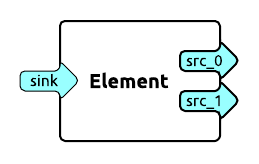
\includegraphics[width=0.5\linewidth]{pics/pic1}
	\caption{ GStreamer pads (sink, src\_0, src\_1)
	}
	\label{fig:ris1}
\end{figure}

Жизненный цикл элементы проводят внутри контейнеров. Контейнер управляет рассылкой сообщений от элемента к элементу, статусами элементов. Контейнеры делятся на два вида: Bin и Pipeline.

Bin -- простой контейнер, который управляет рассылкой сообщений от элемента к элементу которые находятся внутри него. Bin обычно используется для создания группы элементов которые должны совершать какое-либо действие. 
Pipeline является контейнером верхнего уровня, он управляет синхронизацией элементов, рассылает статусы. Например, если pipeline установить статус PAUSED, этот статус будет автоматически разослан всем элементам которые находятся внутри него. Pipeline является реализацией Bin \cite{gstreamer}. 

Источники данных -- это класс плагинов GStreamer, который позволяет читать медиаданные из различных источников, таких как файловая система или аудио-входы звуковой карты. Также, они позволяют получать медиапоток с различных серверов потокового вещания, таких как HTTP (ICECast, ShoutCast), RTSP, RTMP, TCP и UDP. 

Утилита gst-launch-1.0 позволяет запускать GStreamer pipeline без написания кода. Запуск pipeline имеет следующий вид:
gst-launch-1.0 описание-pipeline

Описание pipeline, в свою очередь, делится на описание элементов вида:
element1 property1=value1 property2=value2 ! element2.

Есть элемент типа element1 со свойствами property1 и property2, которые имеют значения value1 и value2 соответственно, и есть элемент типа element2. Символ «!» указывает на то, что выход element1 необходимо соединить с входом element2.
%https://habr.com/ru/post/179167/
% https://docs.gstreamer.com/documentation/
В случае с Raspberry источником видеопотока (element1) является rpicamsrc, который захватывает изображение с RPi камеры. rpicamsrc может выводить видео в виде необработанных кадров или закодированное в формате (M)JPEG или H.264 \cite{gstreamer1}. В качестве element2 будет выступать устройство вывода udpsink,-- это сетевой приемник, который отправляет UDP-пакеты в сеть.
%https://gstreamer.freedesktop.org/documentation/udp/udpsink.html
Для приема и обработки видеопотока на наземной станции может быть использован gscam.

\subsubsection{gscam}
gscam -- ROS драйвер, изначально разработанный для трансляции видеопотока на основе gstreamer через стандартный API камеры ROS. Его можно установить из стандартных репозиториев, предоставляемых менеджером apt или собрать вручную с помощью catkin\_make. gscam может быть запущен и как нода, и как нодлет.

gscam может подключаться к специально отформатированному конвейеру. При условии, что этот конвейер обрабатывает видео в формате RGB. gscam ожидает, что переменная окружения GSCAM\_CONFIG будет содержать gstreamer определение конвейера для его запуска.
gscam получает стрим и публикует 2 топика: /camera/image\_raw(необработанное изображение) и /camera/camera\_info(содержит калибровку камеры и дополнительные данные о конфигурации камеры) \cite{ros}.
% http://wiki.ros.org/gscam

\subsubsection{aruco\_gridboard}
Нода aruco\_gridboard подписывается на топики, публикуемые gscam: топик изображения /camera/image и топик /camera/camera\_info, содержащий параметры камеры. При получении видеопотока aruco\_gridboard распознает карту aruco маркеров, описанную в файле yaml, и публикует статус в топик /vision/status, а полученные координаты в /vision/pose.

Таким образом, видео с Raspberry Pi c помощью gstreamer передается по UDP на ip-адрес наземной станции; нода gscam получает UDP-пакеты и публикует изображение в топики /camera/image\_raw и /camera/camera\_info; aruco\_gridboard подписывается на топики с изображением и информацией о камере и публикует сообщения о положении дрона относительно карты маркеров в /mavros/vision\_pose/pose топик.

%http://www.uco.es/investiga/grupos/ava/sites/default/files/GarridoJurado2014.pdf

